\documentclass{beamer}
\usepackage[orientation=portrait,size=a0,scale=1.4,debug]{beamerposter}
\mode<presentation>{\usetheme{ZH}}
\usepackage{chemformula}
\usepackage[utf8]{inputenc}
\usepackage[english]{babel} % required for rendering German special characters
\usepackage{siunitx} %pretty measurement unit rendering
\usepackage{hyperref} %enable hyperlink for urls
\usepackage{ragged2e}
\usepackage[font=scriptsize,justification=justified]{caption}
\usepackage{array,booktabs,tabularx}

\newcolumntype{Z}{>{\centering\arraybackslash}X} % centered tabularx columns%=
%\sisetup{per=frac,fraction=sfrac}

\title{\huge Stewart platform: \\Kinematics analysis and experiment results}
\author{Trung Kien Tran$^{1}$, Nghia Bao Nguyen Hoang$^{2}$, Duong Trung Ngo$^{2}$, Hoang Viet Dang$^{2}$,\\ Duc Cuong Vu$^{2}$, Danh Huy Nguyen$^{2}$, Tung Lam Nguyen$^{2}$, Trung Kien Nguyen$^{3}$, Vu Nguyen$^{3}$}
\institute{$^{1}$ Institute of Military Technical Automation, Academy of Military Science and Technology \\ $^{2}$ School of Electrical and Electronic Engineering, Hanoi University of Science and Technology\\
$^{3}$ Academy of Military Science and Technology}
\date{\today}

% edit this depending on how tall your header is. We should make this scaling automatic :-/
\newlength{\columnheight}
\setlength{\columnheight}{104cm}

\usepackage{pgfplots}
\pgfplotsset{compat=newest}
\usepackage{float}
\usepackage{booktabs}
\usepackage{multirow}
\usepackage{subcaption}

\usetikzlibrary{calc,angles,patterns,decorations.pathmorphing,decorations.markings}

\begin{document}
\begin{frame}
\begin{columns}
	\begin{column}{.43\textwidth}
		\begin{beamercolorbox}[center]{postercolumn}
			\begin{minipage}{.98\textwidth}  % tweaks the width, makes a new \textwidth
				\parbox[t][\columnheight]{\textwidth}{ % must be some better way to set the the height, width and textwidth simultaneously
					\begin{myblock}{Abstract}
						This paper presents the kinematic analysis, experimental setup, and results of a 6-DOF Stewart platform. The platform is known for high load capacity, precision, and fast response. While inverse kinematics is straightforward, forward kinematics is more challenging. We propose an inverse-kinematics-based optimization method to solve forward kinematics, implemented in C for real-time purpose. The method is also extended to a 7-DOF serial arm for validation. Experiments using EtherCAT and OMRON devices confirm the method’s effectiveness for high-precision applications.
						
						Code available at
						\begin{itemize}
							\item \texttt{github.com/dc-vu/StewartPlatformForwardKinematics}
							\item \texttt{github.com/dc-vu/7DOFsInverseKinematics}
						\end{itemize}
					\end{myblock}\vfill
					\begin{myblock}{State-of-the-art}
						\begin{itemize}
							\item Stewart platform: 6-DOF parallel manipulator with high stiffness and accuracy; widely used in flight simulators, robotic surgery, and precision manufacturing.
							\item Kinematic challenges:
							\begin{itemize}
								\item Inverse kinematics: straightforward and well-studied.
								\item Forward kinematics: nonlinear, coupled, and lacks closed-form solution.
							\end{itemize}
							\item Existing approaches:
							\begin{itemize}
								\item Analytical methods: limited to specific configurations; may yield multiple or no real solutions.
								\item Neural networks: fast inference but require large training datasets and suffer from poor generalization.
								\item Optimization-based methods: formulate FK as a nonlinear least-squares problem; more adaptable to various setups.
							\end{itemize}
							\item Current limitations: real-time implementation and experimental validation are still underexplored in existing studies.
							\item This work: proposes and tests optimization-based FK algorithms (Trust Region \& Levenberg-Marquardt) on real hardware using EtherCAT.
						\end{itemize}
					\end{myblock}\vfill
					\begin{myblock}{Kinematics analysis}
						\begin{figure}
							\begin{minipage}{1\textwidth}
								\centering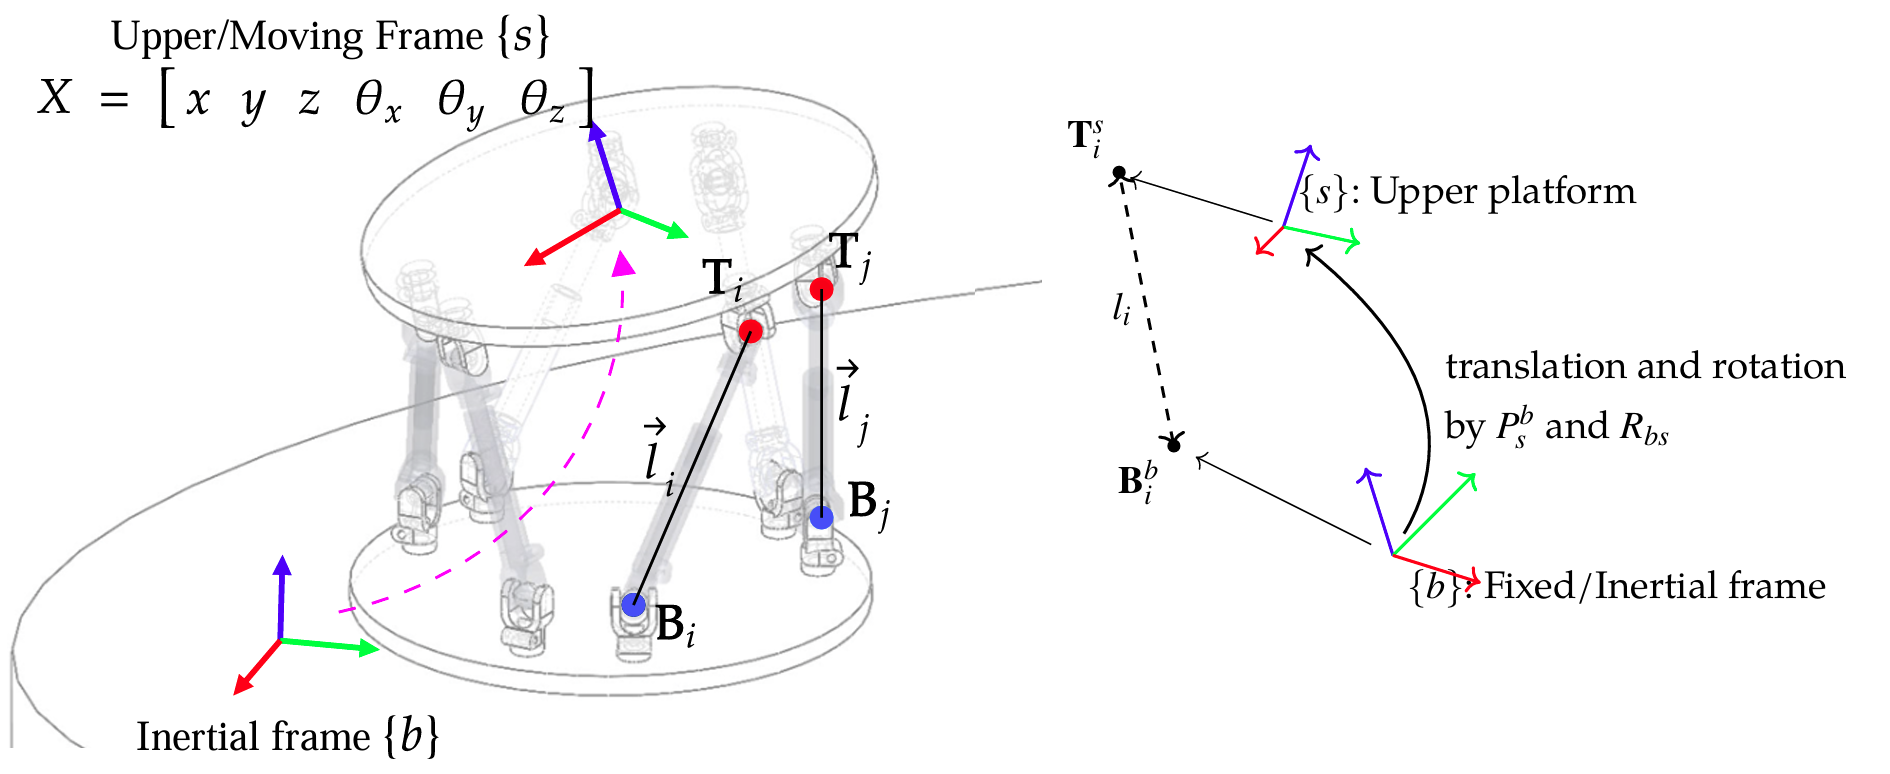
\includegraphics[width=\textwidth]{img/Kinematics.png}
								\caption{Kinematics analysis of Stewart platform. The red, green, and blue arrows are represented as the $Ox$, $Oy$, and $Oz$ axis, respectively.}
								\label{fig: kinematics}
							\end{minipage}
						\end{figure}
						\vspace{1em}
						\begin{itemize}
							\item A Stewart platform consists of 6 legs connecting a fixed base frame $\{b\}$ and a moving frame $\{s\}$ (Figure \ref{fig: kinematics}).
							\item Lower joints $B_i$ and upper joints $T_i$ are fixed in respective frames; leg lengths $l_i = \|L_i\|$ depend on pose $X = [x, y, z, \theta_x, \theta_y, \theta_z]^\top$.
							
							\item \textbf{Inverse Kinematics:} Given $X$, leg vectors
							\[
								L_i = P + T_i R_{bs}(\Theta) - B_i \text{ yield } l_i = \|L_i\|
							\]  
							
							$\to$ IK is well-posed and analytical.
							
							\item \textbf{Forward Kinematics:} Given $\mathcal{L}_r = [l_1, ..., l_6]^\top$, solve 
							\[\mathcal{L}(P, \Theta) = \mathcal{L}_r\]
							
							\item \textbf{Optimization Formulation:}
							\[
							g(\mathcal{L}_r) = \arg\min_{P, \Theta} \|\mathcal{L}(P, \Theta) - \mathcal{L}_r\|
							\]
							\item Trust Region and Levenberg-Marquardt methods are used for solving FK. C and Python implementations are available on GitHub.
							
							\item \textbf{Note:} Optimizers may converge to local minima. Validation of the solution is required.
							
							\item \textbf{Extension:} The same optimization principle is applied to solve inverse kinematics of a 7-DOF serial arm.
						\end{itemize}
					\end{myblock}\vfill
		}\end{minipage}\end{beamercolorbox}
	\end{column}
	\begin{column}{.57\textwidth}
		\begin{beamercolorbox}[center]{postercolumn}
			\begin{minipage}{.98\textwidth} % tweaks the width, makes a new \textwidth
				\parbox[t][\columnheight]{\textwidth}{ % must be some better way to set the the height, width and textwidth simultaneously
					\begin{myblock}{Numerical evaluation}
						
						\begin{itemize}
							\item \textbf{Results on Stewart Platform (6-DOF):}
							\begin{itemize}
								\item Levenberg-Marquardt is $>50\times$ faster than Trust Region
								\item Reduces iterations by $>100\times$
								\item Higher robustness and accuracy
							\end{itemize}
							
							\item \textbf{Results on Serial Arm (7-DOF):}
							\begin{itemize}
								\item $30\times$ faster in execution time
								\item $50\times$ fewer iterations
								\item Lower error and no failure observed
							\end{itemize}
						
							\item \textbf{Hardware:} Laptop CPU Ryzen 7 5600U @ 1.7GHz
						\end{itemize}
					\vspace{1em}
					\begin{minipage}{0.65\linewidth}
						{
							\fontsize{20pt}{30pt}\selectfont
							\begin{table}
								\centering
								\caption{Comparison between Trust Region and Levenberg-Marquardt methods on Inverse/Forward kinematics problems}
								\label{tab: performance}
								\renewcommand{\arraystretch}{1.2}
								\begin{tabular}{c c cc cc }
									\hline
									\hline
									\multirow{2}{*}{\textbf{Method}} & \multirow{2}{*}{\textbf{Metric}} & \multicolumn{2}{c }{\textbf{Stewart platform (6DOFs)}} & \multicolumn{2}{c }{\textbf{7DOFs serial robot arm}} \\
									% \cline{3-6}
									& & Near solution & Home position & Near solution & Home position \\
									\hline
									
									\multirow{4}{*}{\textbf{Trust Region}} 
									& Avg. time ($\mu$s)   & 949.334   & 1157.346   & 3526.206   & 3763.735     \\
									& Avg. error           & $6.8 \times 10^{-3}$ & $15.9 \times 10^{-3}$ & $2.86 \times 10^{-3}$ & $11.6 \times 10^{-3}$ \\
									& Avg. iteration       & 148.26     & 179.5      & 186.32     & 197.67    \\
									& Failures             & 0\%        & $\approx$ 0.5\%        & 0\%        & 0\%       \\
									\hline
									\multirow{4}{*}{\textbf{LM}} 
									& Avg. time ($\mu$s)   & 14.118     & 23.243     & 109.255    & 151.502   \\
									& Avg. error           & $88 \times 10^{-6}$ & $47 \times 10^{-6}$ & $66 \times 10^{-6}$ & $61 \times 10^{-6}$ \\
									& Avg. iteration       & 1.003      & 1.994      & 4.594      & 6.797     \\
									& Failures             & 0\%        & 0\%        & 0\%        & 0\%       \\
									\hline
									\hline
								\end{tabular}
							\end{table}
						}
					\end{minipage}
					\hfill
					\begin{minipage}{0.30\linewidth}
						\begin{figure}[H]
							\centering
							\scalebox{2}{\fontsize{12pt}{20pt}\selectfont
								\begin{tikzpicture}
									\begin{axis}[
										axis lines=middle,
										% xlabel={$x$}, ylabel={$y$},
										xmin=-3.5, xmax=8,
										ymin=-3, ymax=10,
										samples=200,
										domain=-3.5:4.5,
										legend style={at={(0.5,-0.15)},anchor=north},
										xtick=\empty, ytick=\empty,
										axis line style={->}
										]
										
										% Define the function f(x)
										\addplot[blue, thick, domain=-3.5:4.5] {-(x + 0)*(x + 1)*(x - 1) + 2*3*1} node[pos=0.85, above right] {$f(x)$};
										
										% Define the absolute value of f(x)
										\addplot[red, thick, domain=-3.5:4.5, dashed] {abs(-(x + 0)*(x + 1)*(x - 1) + 2*3*1} node[pos=0.9, above right] {$|f(x)|$};
										
										% Coordinates of local extremum xl and zero crossing xg
										\coordinate (xl) at (axis cs:-0.577, 6-0.38);
										\coordinate (xg) at (axis cs:2,0);
										
										
										\coordinate (t0) at (axis cs:2.6,8.976);
										
										% Mark xl (local extremum of f)
										\filldraw[blue] (xl) circle (2pt);
										\node[below] at (xl) {$x_l$ (local min.)};
										
										% Mark xg (global extremum of |f|)
										\filldraw[red] (xg) circle (2pt);
										\node[below left] at (xg) {$x_g$ (global min.)};
										
										\node[left] at (t0) {\color{red}$t_0$};
										
										\addplot[green, thick, domain=1.8:4.5, dashed] {-(x-0.5 + 0)*(x-0.5 + 1)*(x-0.5 - 1) + 2*3*1} node[pos=0.13, above right] { $f(x)\, \mathrm{ at }\, t_0 + \Delta t$};
										
										% Define the absolute value of f(x)
										\addplot[blue, thick, domain=1.8:4.5, dotted] {abs(-(x-0.5 + 0)*(x-0.5 + 1)*(x-0.5 - 1) + 2*3*1} node[pos=0.1, above right] { $|f(x)|\, \mathrm{ at }\, t_0 + \Delta t$};
										
										% Vertical line from xg to intersection with green curve
										\draw[dashed] (axis cs:2, 0) -- (axis cs:2, 4.125);
										\node[right] at (axis cs:2, 4.125) { $\leftarrow$ initial guess};
										\filldraw[black] (axis cs:2, 4.125) circle (1pt);
										
									\end{axis}
								\end{tikzpicture}
							}
							\caption{Local and global minimum illustration.}
							\label{fig: optimization}
						\end{figure}
					\end{minipage}
					\begin{itemize}
						\item \fontsize{23pt}{30pt}\selectfont The performance of the proposed algorithm could be significantly increased by using the flag \texttt{-O2} when compiling by \texttt{gcc}. 
						
						The average time of Levenberg-Marquardt can reduce to about 2-3 $\mu$s without failures.
					\end{itemize}
					\end{myblock}\vfill
				
					\begin{myblock}{Experiment setup and results}
						\begin{itemize}
							\item \textbf{Robot:} 6-DOF Stewart platform actuated by 6 linear cylinders.
							\item \textbf{Actuation:}
							\begin{itemize}
								\item Each cylinder is driven by an OMRON AC servo motor.
								\item Upper joints: 3 DOFs; lower joints: 2 DOFs.
								\item Prismatic joints allow full 6-DOF spatial motion.
							\end{itemize}
							\item \textbf{Control System:}
							\begin{itemize}
								\item Motors are controlled via OMRON servo drivers (EtherCAT slaves).
								\item Master: OMRON NJ501-1300 PLC.
								\item Communication with monitoring PC via Ethernet.
							\end{itemize}
						\end{itemize}
						\vspace{1em}
						\begin{figure}
							\begin{minipage}{\textwidth}
								\centering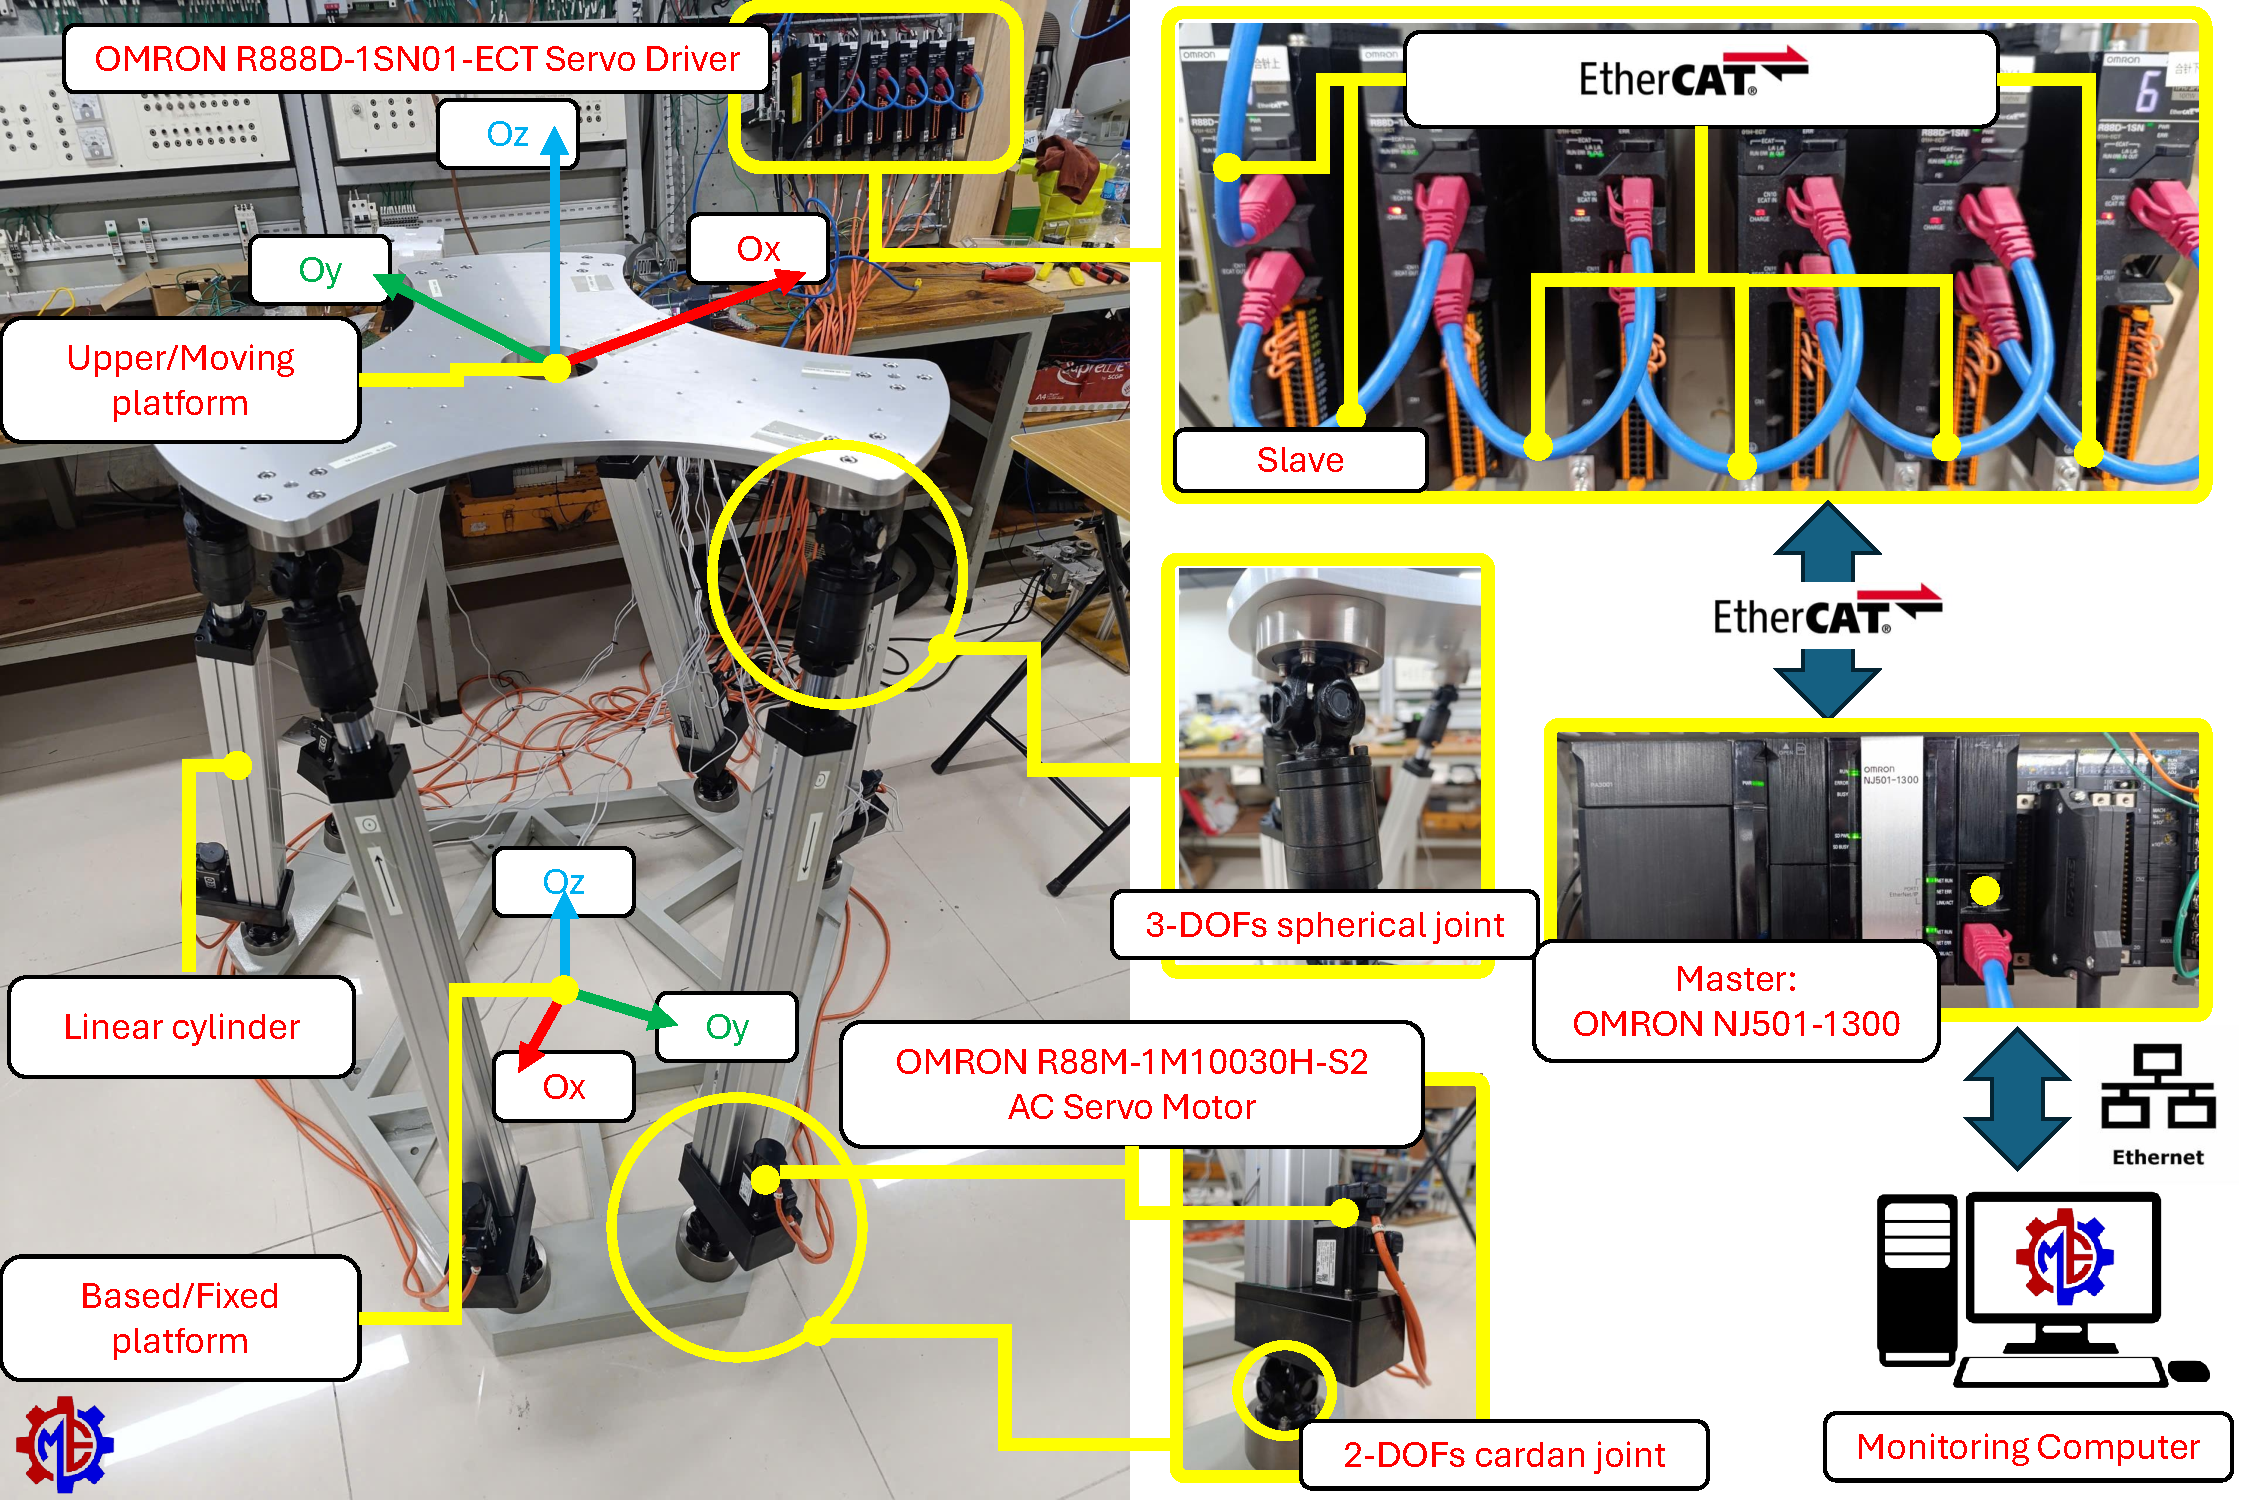
\includegraphics[width=0.9\textwidth]{img/experiment_setup.pdf}
								\caption{Experiment setup of Steawrt platform at Motion Control and Applied Robot Laboratoty (MoCAR, HUST).}
							\end{minipage}
						\end{figure}
						\vspace{1em}
						\begin{itemize}
							\item Experiment results
						\end{itemize}
						\begin{figure}
							\begin{subfigure}{0.48\textwidth}
								\centering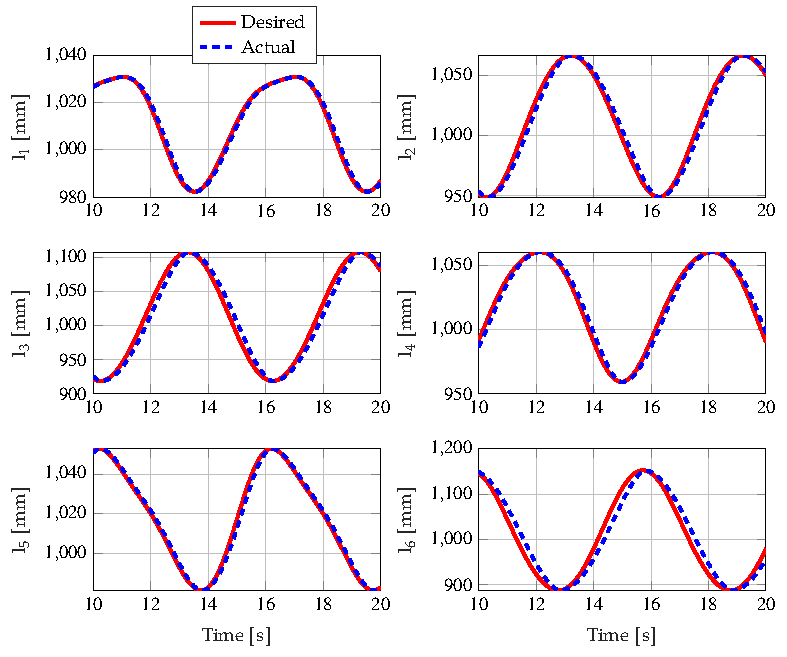
\includegraphics[width=\textwidth]{img/result1.pdf}
							\end{subfigure}
							\hfill
							\begin{subfigure}{0.48\textwidth}
								\centering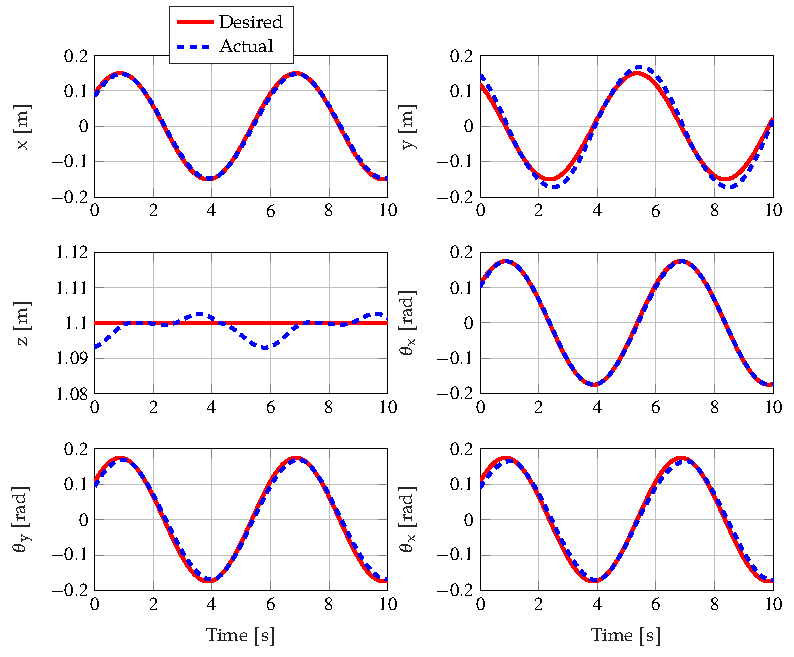
\includegraphics[width=\textwidth]{img/result2.pdf}
							\end{subfigure}
							\caption{Experiment results of leg length tracking performance of servo controllers and forward kinematics calculated.}
						\end{figure}
					\end{myblock}\vfill
				
%					\begin{myblock}{References}
%						\footnotesize
%						\bibliographystyle{abbrv}
%						\bibliography{./bib}
%					\end{myblock}\vfill
		}\end{minipage}\end{beamercolorbox}
	\end{column}
\end{columns}
\end{frame}
\end{document}
